\chapter{GPU Implementations}
\label{chap:imp}

In this chapter, all GPU implementations will be explained in detail, both the preliminary studies done to motivate the algorithmic choices made in WARP and of those in WARP itself.

\section{Preliminary Studies}
\label{sec:prelim}

Before any serious coding efforts were undertaken, a pair of smaller preliminary studies were done to determine the feasibility of doing Monte Carlo neutron transport on GPUs.  The first study was attempting to to perform a simple, 2D, mono-energetic scattering game on a GPU.  The second study was a test of the OptiX framework to see if it could handle randomized ray tracing and still have acceptable performance.

\subsection{2D Scattering Game}

\begin{figure}[h!] 
  \centering
    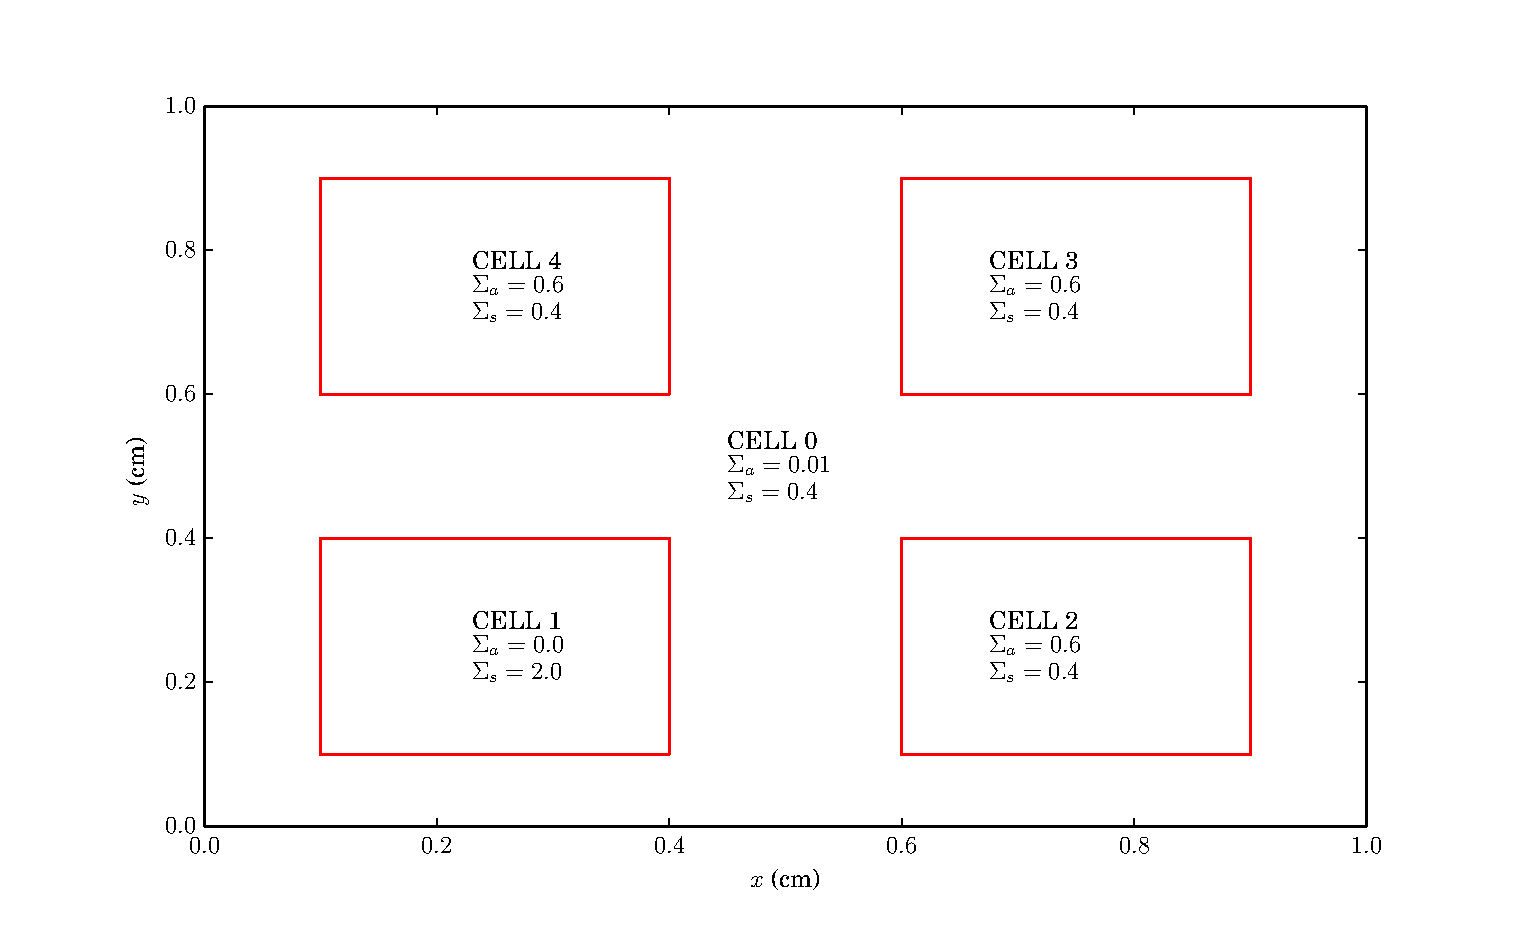
\includegraphics[width=0.8\textwidth]{graphics/prelim_geom.eps}
     \caption{The 2D geometry of the scattering test. \label{prelim_geom} }
\end{figure}

The goal of the 2D mono-energetic scattering game was to highlight if a sorted or unsorted event-based algorithm was best for controlling thread divergence on a GPU, to the see the relative performance of the history- and event-based GPU implementations to an identical serial CPU version, and to determine if the performance of the CUDPP (CUDA Parallel Primitives) library is adequate for use in WARP.   A set of three GPU implementations were written using CUDA C, and a single CPU implementation was written using C.

In the simulation, only two reaction types are possible - scattering and absorption.  Scattering is treated isotropically, and since it is mono-energetic, scattering only serves to change the direction of a particle.  The geometry of the game is simple in order to highlight how the reaction divergence is handled rather than how geometry routines effect performance.   The geometry used in the game is shown in Figure \ref{prelim_geom}.  There are five different cells, which are all square, and particles can only move in the $x$-$y$ plane.  Each cell has different reaction cross sections, and cell 0 extends to infinity, but has a nonzero absorption cross section so particles cannot scatter forever.  Particles are initialized with a uniform, random distribution in cell 1, which has no absorption cross section so they must cross a cell boundary at least once.  Since the cells are few and square, the ``where am I?'' operation that determines the cell number (and therefore the cross sections) each particle is in can be done with simple, hardcoded logic comparisons.

As particles scatter, they start to be absorbed and their histories are terminated.  This means they are no longer transported, and their data should no longer be accessed.  Here is where the GPU implementations start to differ from one another.  The task-based implementation performs the transport from a one particle per thread standpoint.  When the transport kernel is launched, each thread contains a while-loop that transports a particle until it terminates and the thread returns.  If more histories are requested than the maximum thread number, transport is performed in batches.  The diagram of the simple task-based algorithm used is shown in Figure \ref{prelim_alg_task}.  The CPU version of the code also uses this algorithm.

\begin{figure}[h!] 
  \centering
    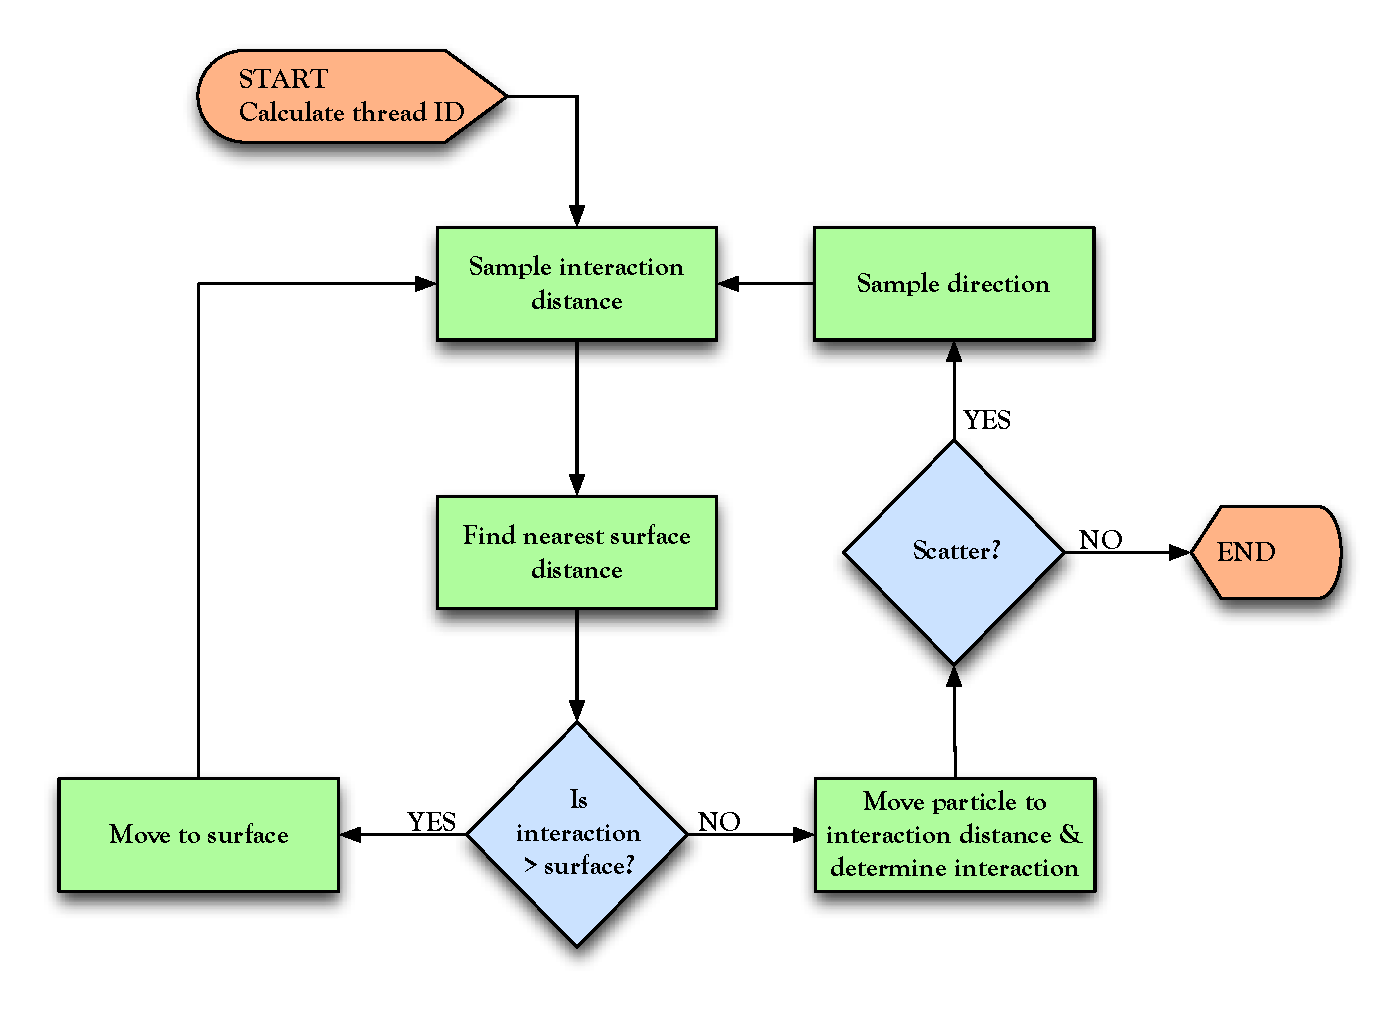
\includegraphics[width=0.7\textwidth]{graphics/prelim_alg_task.eps}
     \caption{The task-based algorithm used in the 2D scattering study. \label{prelim_alg_task} }
\end{figure}

The event-based algorithm performs the same operations on the data as the task-based algorithm, of course, but the operations are now carries out over all the particle data simultaneously in parallel.  Now, each kernel does \emph{not} contain a while loop.  The while loop is now on the CPU host, the drawbacks to which are discussed later.  Each kernel performs a single, simple task on the entire particle dataset in one step.  An analogy can be made with homework grading.  The task-based algorithm is like grading a single student's homework in its entirety, then moving on to the next student's.  The event-based approach is like grading a single \emph{problem} for \emph{every student}, then moving on to the next problem.  This makes the transport loop \emph{data parallel}, which GPUs need to keep warps coherent. 

\begin{figure}[h!] 
  \centering
    \includegraphics[width=0.7\textwidth]{graphics/prelim_alg_event.eps}
     \caption{The event-based algorithm used in the 2D scattering study. \label{prelim_alg_event} }
\end{figure}

Two different implementations were made using a event-based algorithm, one which uses the CUDPP compaction to remap threads to non-terminated (active) data, and one which does not.  In the non-remapping version, threads simply return if they access data belonging to a terminated particle.  In the remapping version, the number of threads launched is equal to the number of active particles left in the dataset, not the size of the dataset itself.  They access a remapping vector, which transforms their thread ID to be one which still contains active data.  Figure \ref{remapping} shows how the remap vector transforms the initial thread ID to an active ID.  The CUDPP compaction function does just this - it takes an input vector and a valid flag vector and returns a new vector containing only the valid elements, preserving the order which they are in.  For this test, the input vector is the thread ID vector (tid[i]=i), and the flag vector contains a 1 if a particle is unterminated and a 0 if it is not.  The compact function then returns a remapping vector which is as long as the number of unterminated particles which contains the indices of the unterminated data.

\begin{figure}[h!] 
  \centering
    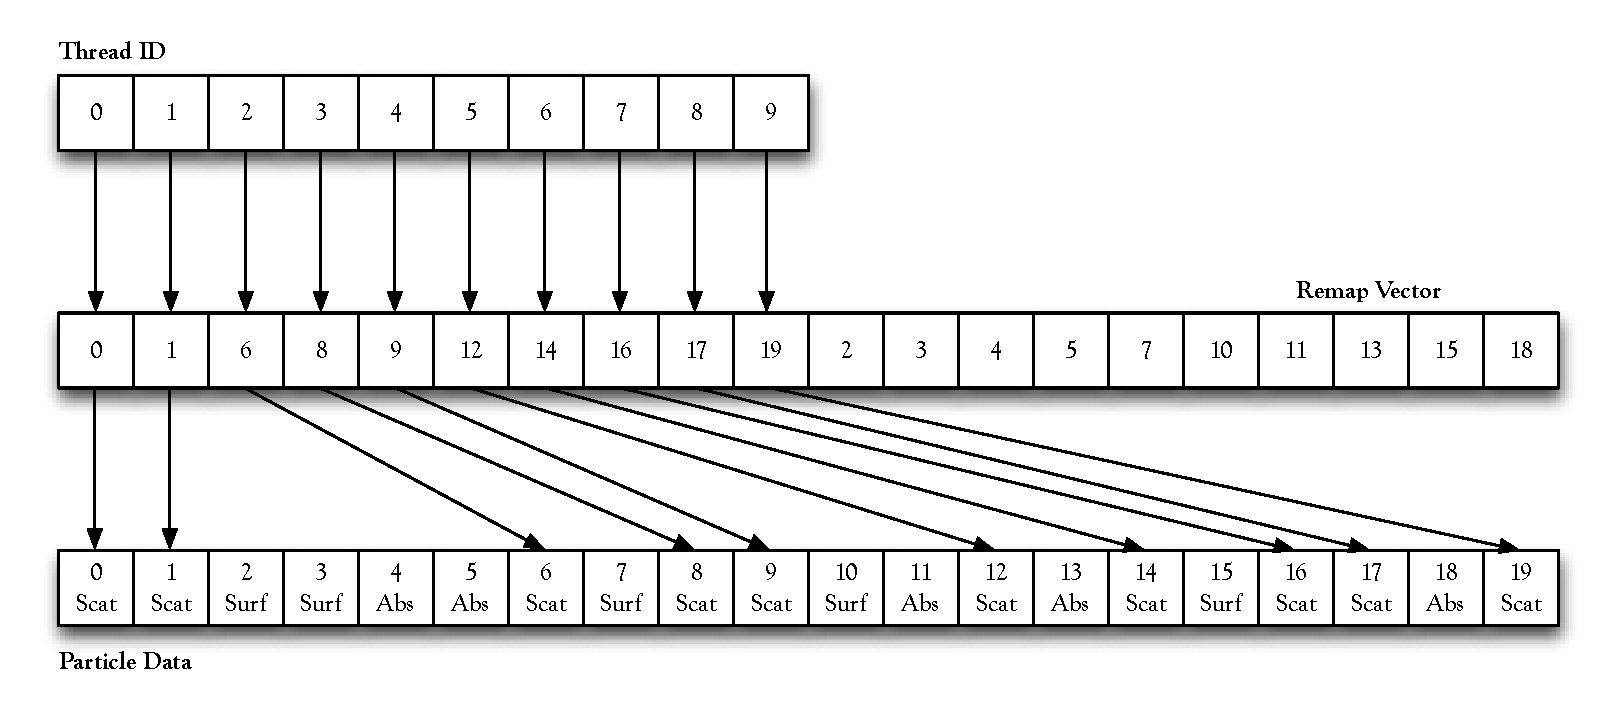
\includegraphics[width=0.8\textwidth]{graphics/remapping_horiz.eps}
     \caption{Mapping thread IDs to active data through a remapping vector \label{remapping} }
\end{figure}

Figure \ref{prelim_speedup} shows the speedup factors, $F_s=t_\mathrm{CPU}/t_\mathrm{GPU}$, of the GPU implementations over the CPU implementation versus the number of particles run.  This benchmark was run on a server with a 8-core AMD Opteron 6128 CPU clocked at 2.0GHz, and there different NVIDIA cards - a Tesla K20, a Tesla C2075, and a GeForce 480 GTX.  The following results were obtained from running the GPU implementations on the Teslta K20.  The task-parallel implementation performs best, with a maximum speedup of around 29x.  The remapping implementation has the next best performance, with about a 20x speedup over the CPU.  It's performance plateaus, unlike the batched event-based implementation.  It's performance departs from the remapping implementation at $10^5$ particles and even starts to deteriorate between $10^6$ and $10^7$ particles.  This is due to the transport having to be done in batches at this point.  The simulations were done on a Tesla C2075 card, which has Fermi architecture and a maximum block number of 65,536 for a 1D grid.  Multiplying this by 128 or 512 threads per block gives maximum total number of threads of 8,388,608 and 33,554,432, respectively.  These numbers are where the batching implementation must break the transport into multiple batches.  This is also where the task-based implementation must break transport into batches, but the effect is unnoticeable since it only implies a second kernel launch instead of hundreds more.  This limit was lifted in devices with compute capability of 3.0 and up, where the maximum 1D grid size was increased to ($10^{27}-1$) \cite{cuda}.  The speedup plot also shows another important feature - that speedup plateaus at a large number of histories.  This is due to the car'd ability to hide memory latencies through pipelining when there are many many active threads.  

The number of threads per block seems to make little difference in the event-based implementations, but makes a very large difference in the task-based implementation.  Increasing the number of threads per block from 128 to 512 reduces the performance from a 28x speedup to a 20x speedup, comparable to the event-based implementations.  The reason for this happening is most likely registers spilling to local memory since there are more threads resident in a multiprocessor and more variables need to be stored in the registers.

\begin{figure}[h!] 
  \centering
    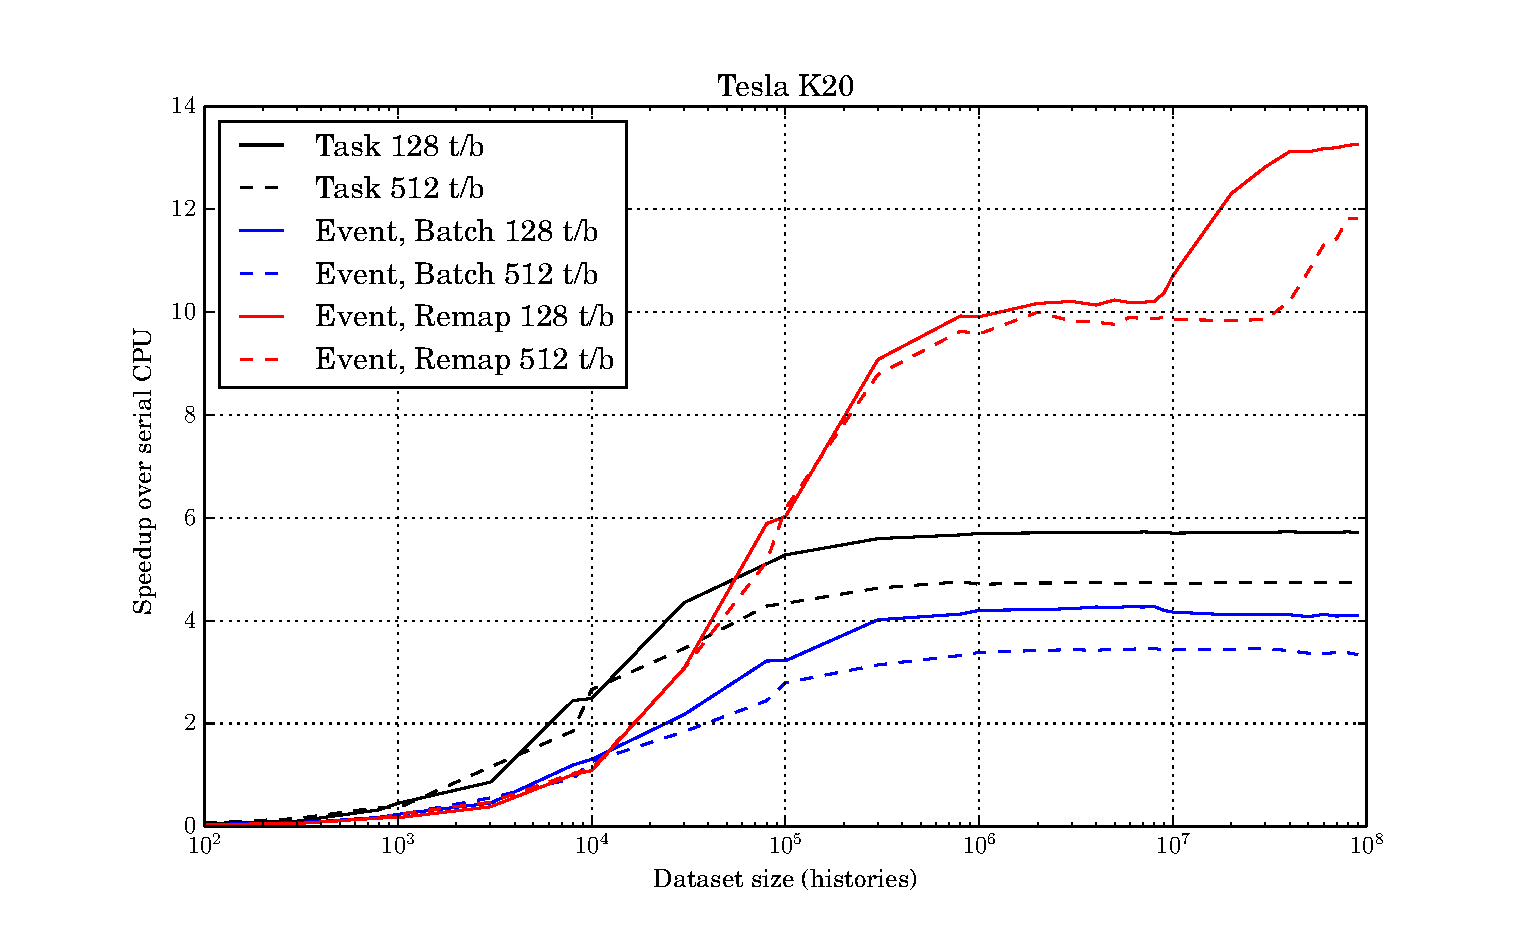
\includegraphics[width=0.8\textwidth]{graphics/prelim_speedup_k20.eps}
     \caption{Speedup factors of the GPU implementations over the CPU implementation on a Tesla K20. \label{prelim_speedup} }
\end{figure}

\begin{figure}[h!] 
  \centering
    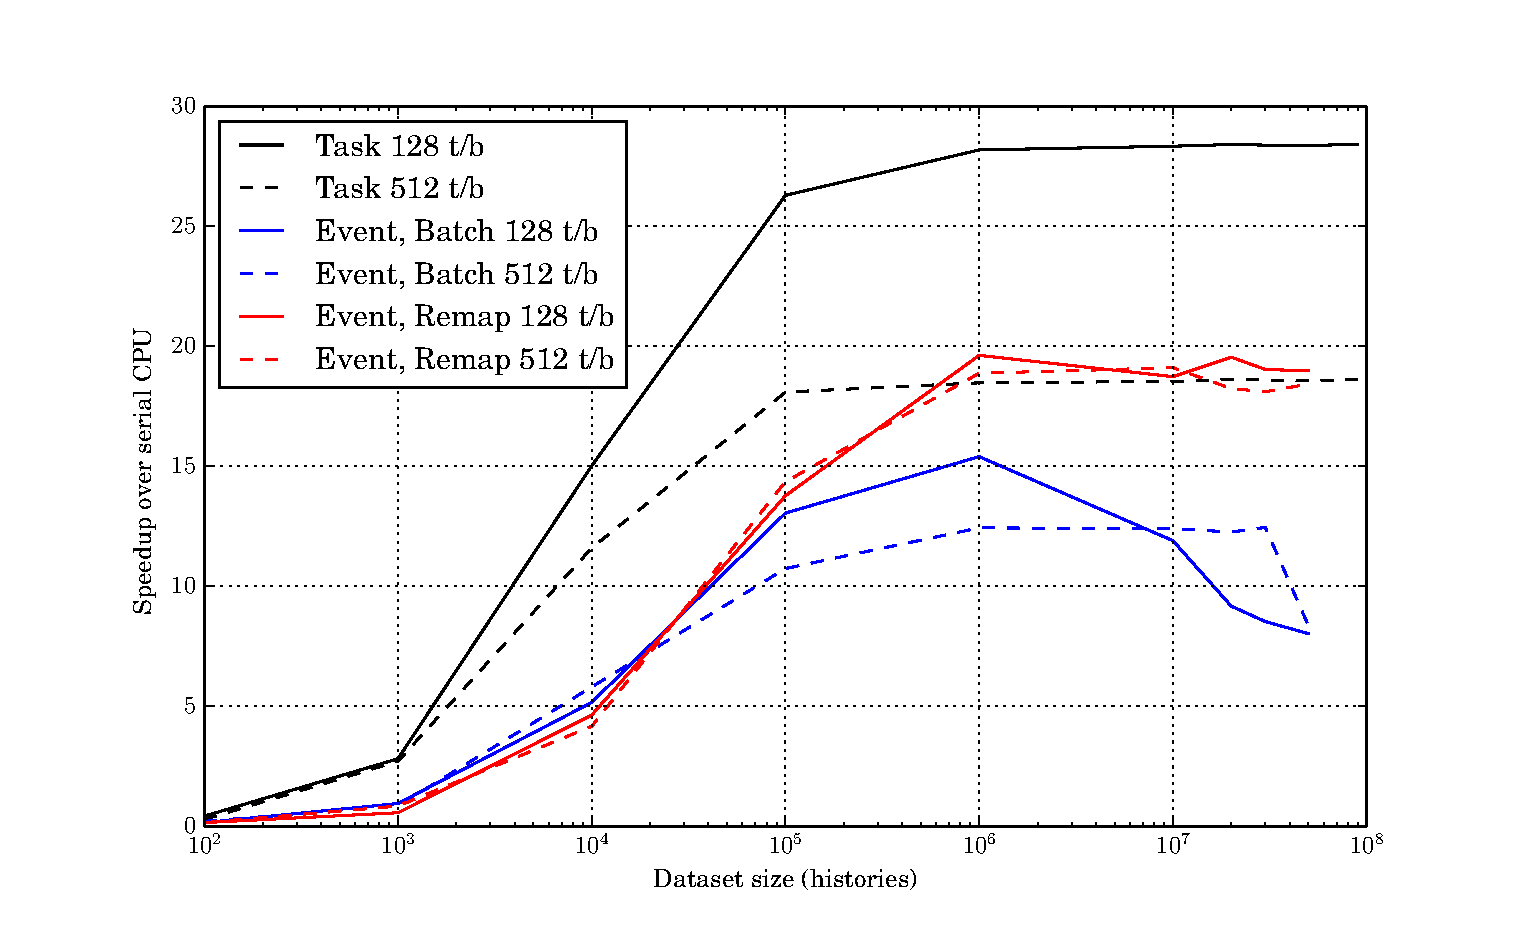
\includegraphics[width=0.8\textwidth]{graphics/prelim_speedup_old.eps}
     \caption{Speedup factors of the GPU implementations over the CPU implementation on a Tesla C2075 (UPDATE FOR $\Sigma$=.01). \label{prelim_speedup} }
\end{figure}

Figure \ref{prelim_active} shows the number of active histories per transport iteration for the batches and remapping implementations.  Since the remapping implementation eliminates all references to terminated particles, the data loaded into the threads blocks is all active and no threads return without doing work.  The figure clearly shows that the blocks are kept full until the end of the simulation when the remain number of particles becomes less than the maximum number of threads.  It also shows how quickly particles are depleted from the blocks.  In this simple case, most interactions happen in cell 0 by far, and particles are absorbed almost identically to \eqref{depleted}, where $i$ is the iteration number and $\Sigma_a/\Sigma_t$ is the absorption probability in cell 0.   Figure \ref{prelim_active} does not reflect the time taken by each iteration, however.  The iterations with more particles take longer than those with fewer for both implementations.  More particles are transported per time in full iterations, however, as evidenced by the greater speedups of the remapping algorithm in Figure \ref{prelim_speedup}.

\begin{equation}
\label{depleted}
\frac{N}{N_0}=\exp \left(-\frac{\Sigma_a}{\Sigma_t} i \right)
\end{equation}

\begin{figure}[h!] 
  \centering
    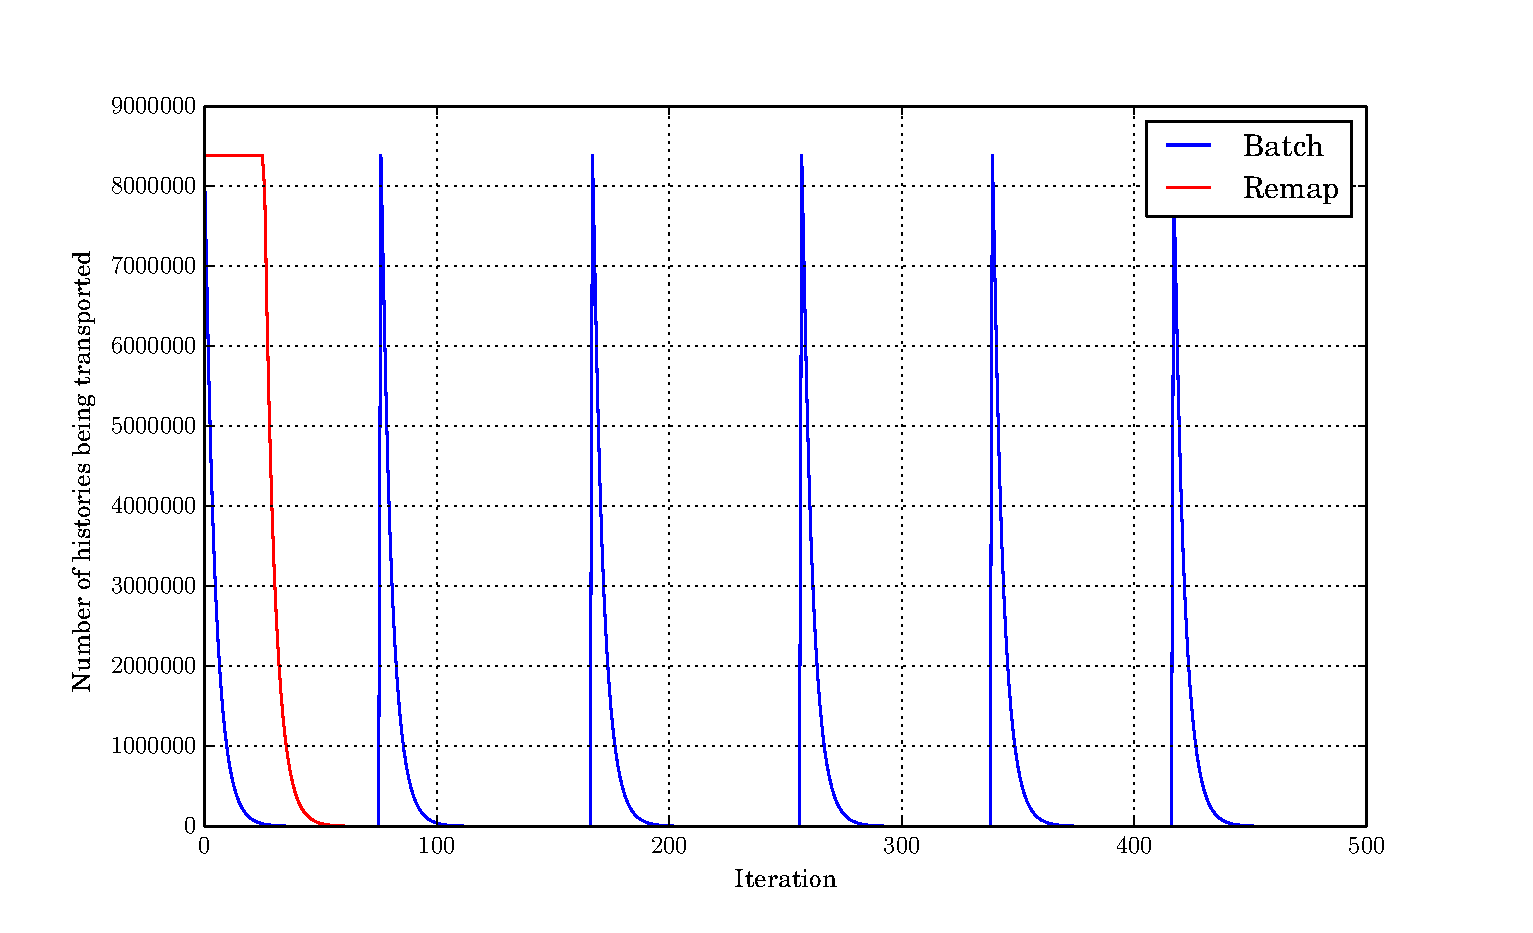
\includegraphics[width=0.8\textwidth]{graphics/prelim_active.eps}
     \caption{The number of actively transporting threads for the event-based GPU implementations. \label{prelim_active} }
\end{figure}

The most likely reasons that the task-based implementation outperforms the event-based is due the simplicity of the problem and the communication and setup overhead associated with many kernels being launched from the host.  Since the problem is so simple, all the data fits into local memory and the latencies associated with accessing global memory often are hidden.  The purpose of this study was to eliminate memory transaction and only focus on thread divergence, but memory transactions will have a very large impact when real cross sections and geometries are used.  Also only having two reactions means threads only diverge when they terminate.  WARP will have many reactions types to deal with, and divergence will be a greater problem.  This also allows threads in a block to almost always be in the same step of the transport algorithm, further eliminating divergence implicitly.  Despite this, the study does show that control flow divergence is greatly reduced by using an event-based algorithm, as shown by Figure \ref{prelim_divergence}.  The overhead of calling kernels many times in the event-based implementations is most likely the reason for the poorer performances.

\begin{figure}[h!] 
  \centering
    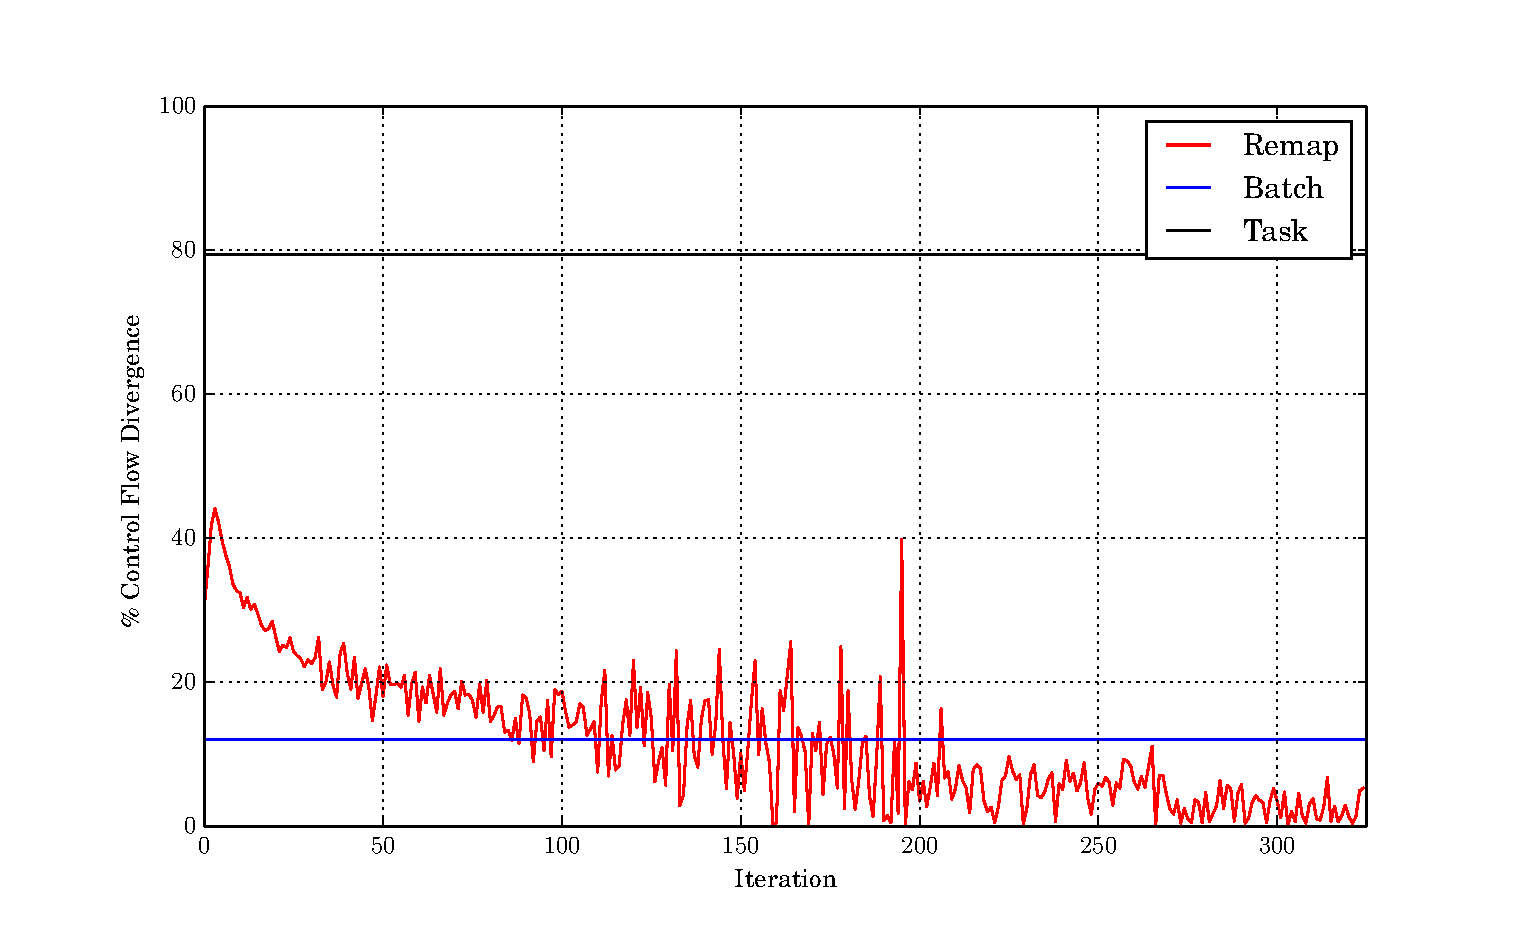
\includegraphics[width=0.8\textwidth]{graphics/prelim_divergence.eps}
     \caption{The \% of control flow divergence of the task- and event-based GPU implementations (UPDATE). \label{prelim_divergence} }
\end{figure}

Another consideration pointed out by this study is that library use and the task-based algorithm are incompatible.  Libraries currently available for the GPU carry out a single task on a dataset, they are not coded for single-thread operation and must be launched as their own kernels.  Having threads in different states wouldn't allow the library routines to be dropped in and carried out consistently across all the active particle data.  Also, much of the performance from optimized algorithms comes from thread blocks cooperating, and using a task-based algorithm would be like treating each SM as a separate CPU (using a stack-popping method) and would minimize the benefits of divide-and-conquer algorithms.

From this preliminary 2D mono-energetic scattering study, it can be concluded that using an event-based algorithm with a compaction/sort algorithm to eliminate terminated particles from being accessed by thread blocks drastically reduces control flow divergence and keeps warps coherent.  There is a cost for adopting this algorithm, however, namely the overhead of kernel launches.  How these factors compete in WARP will be shown in the results in Chapter \ref{chap:results}.  WARP will adopt the event-based algorithm in hopes that thread coherency and its benefits (maximal load coalescing, little warp serialization) will outweigh launch overhead in when real data is used, as well as to allow library usage in complicated parallel tasks.

\subsection{Ray Tracing with OptiX}

Another preliminary study was preformed in order to determine the performance of OptiX when ray tracing from randomized points as well as to find the optimal OptiX configuration for WARP.  In rendering, rays are initialized in a uniform array, but the flexibility from writing custom ray generation program in OptiX allows for arbitrary starting points and directions to be used.

\subsubsection{Point-in-Polygon / Material Query}

\begin{figure}[h!] 
  \centering
    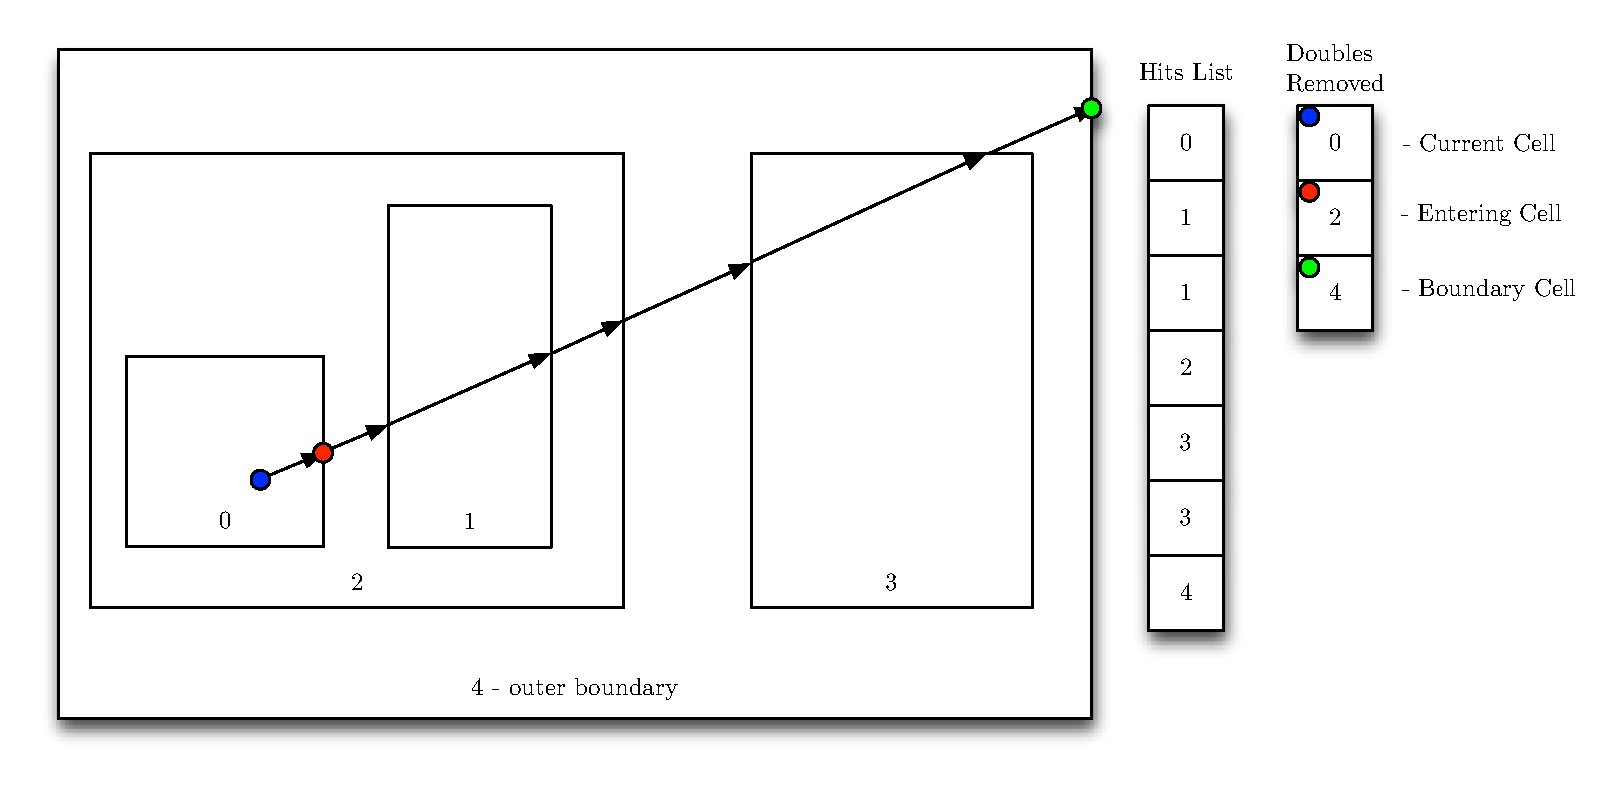
\includegraphics[width=1.0\textwidth]{graphics/whereami.eps}
     \caption{The point-in-polygon-like algorithm for determining the entering cell number by using ray tracing \label{whereami} }
\end{figure}

An important job for the geometry routine in a Monte Carlo neutron transport code is to determine the cell and material IDs of a particle based only on it's coordinates.  This is very important in Woodcock tracking, since surface intersections are not calculated and this material query it is the only place where geometrical information enters into the simulation.  In WARP and other ray-tracing codes, material information is only updated when a neutron sampled interaction distance is greater than the near surface distance.  In this situation, the neutron is placed on the boundary, the material information is updated for the new material, and the interaction distance is sampled again using the same direction of flight as before.  WARP will use and algorithm to determine the entering cell number by using ray tracing, since all the geometrical information is stored in the OptiX context.  This will also mean the material query will be able to take advantage of the OptiX acceleration structures, and should scale well (logarithmic).

The material query algorithm is shown in Figure \ref{whereami}.  An ordered list of surface intersections is generated by iteratively ray tracing and adding the closest surface number to the hit list.  Tracing is terminated when a predefined outer cell is intersected which all other cells are inside of.  Since all surfaces are closed, the ray will intersect any cell surface twice that it isn't nested in.  When the list is made, the double entries are removed, which yields a list of cells the neutron is nested in.  The first entry will be its current cell and the second entry will be the cell it is entering into.  It is important to make the scene epsilon an appropriate value for the geometry if this algorithm is to be used effectively.  The scene epsilon determines the minimum intersection distance possible, i.e. the distance away from the source point which intersections are allowed to occur.  This prevents self-intersections from happening due to numerical inaccuracies.  The mathematical cell descriptions are exact, but the number representing them are not, and if they are treated as exact, a situation can occur where a neutron is placed at a boundary, but it is actually slightly behind the boundary due to floating-point roundoff.  When the next trace is started, the ray intersects the boundary it has already intersected with instead of tracing into the next cell.  Giving OptiX a scene epsilon guarantees the trace starts after the very near boundary, and accurate results are calculated.

This algorithm is very similar to the ray casting point-in-polygon algorithm which determines if a point is inside or outside of an arbitrary polygon by counting the number of times it crosses a surface.  An even number means it is outside and an odd number means it is inside.  This algorithm is almost the same, but it keeps track of cell numbers instead of binary logic for one surface.  This way, the nesting of a neutron can a be determined and the entering cell can be found.  Both of these algorithms take advantage of the cell being closed, and in this sense is similar to Gauss's Law or the divergence theorem which states the flux integrated around a surface will be nonzero only if the surface contains a source.  This material query algorithm is like a discrete, single field line version where the neutron's position is the source point and the cell boundaries are the integrating surfaces.

An important consideration in this type of geometrical representation is that the volume of a cell is \emph{always} the spatial intersection of the space inside of the cell with space outside any cells nested inside it.  For example, if two cube cells were specified to be centered at the origin with cube 2 completely encompassed by cube 1, the space in-between cube 1 and cube 2 would belong to cell 1 while the space inside cube 2 would all belong to cube 2.

\subsubsection{Instancing}

\begin{figure}[h!] 
  \centering
    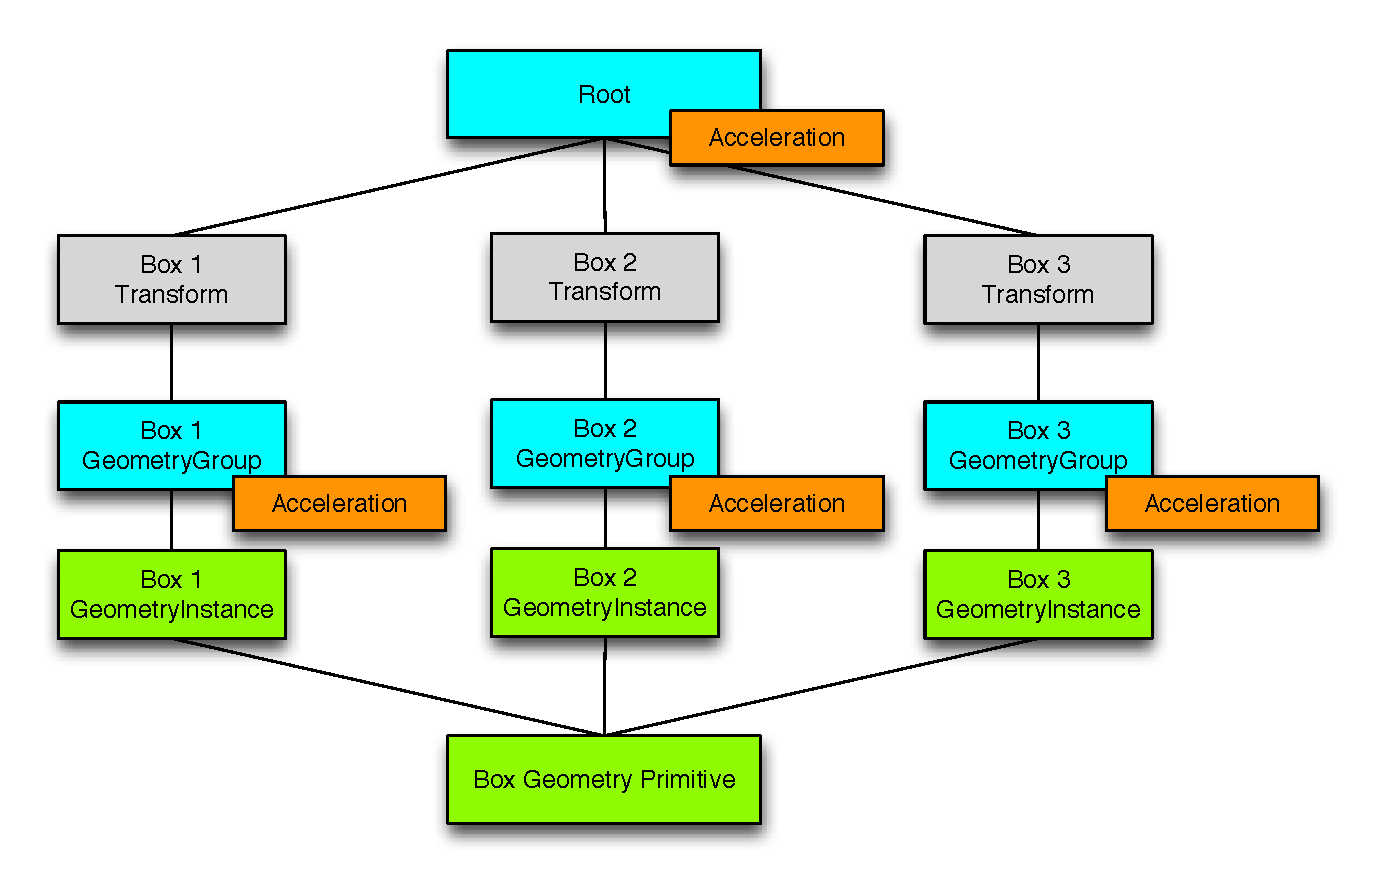
\includegraphics[width=0.8\textwidth]{graphics/transform_instancing.eps}
     \caption{The OptiX node graph using transform instancing \label{transform_instancing} }
\end{figure}

Nuclear reactors can have very complicated geometries, but they basically rely a simple shapes that are repeated in arrays.  There are a few ways in which identical cells can be instanced in OptiX.  the first and most convenient is to define a single primitive in it's own coordinate system, then use a transform node (shown in Figure \ref{node_graph}) in the OptiX node graph to transform the primitive to it's actual position via an affine transformation matrix.  The resulting node graph is shown in Figure \ref{transform_instancing} for a scene that has three boxes in it.  As a reminder, a GeometryInstance objects ties a hit program to the spatial geometry data in the geometry primitive object, acceleration objects are attached to all group objects, and transform objects can only have children that are Group or GeometryGroup objects which is why each GeometryInstance must have its own GeometryGroup.

Transform instancing is convenient since only a single primitive needs to be defined.  If another instance is needed, one can simply apply a transform matrix to it and all the work is done by OptiX.  This scheme has a lot of overhead, however, since each instance has it's own group and its own acceleration object, producing a deeper node graph than necessary.

\begin{figure}[h!] 
  \centering
    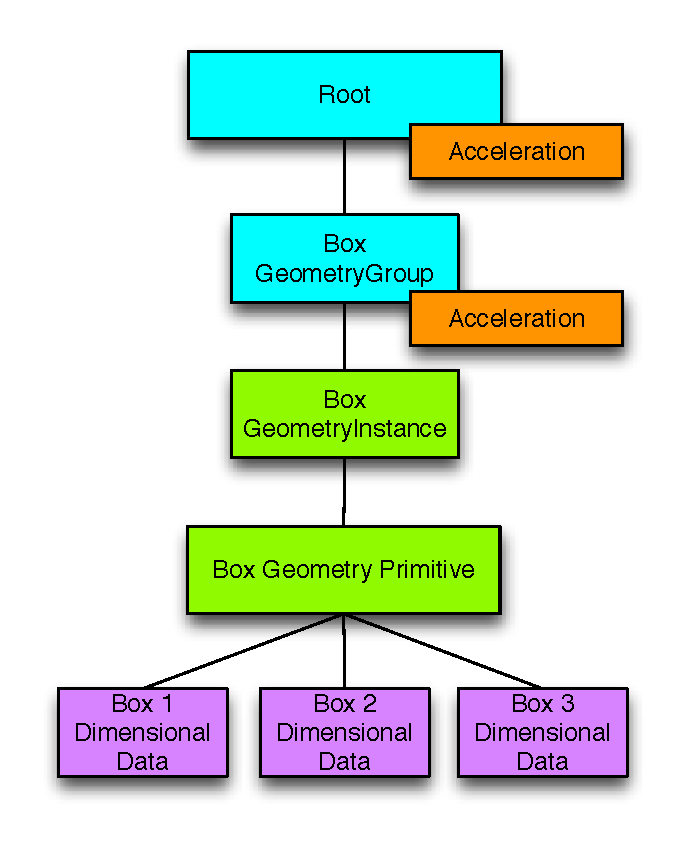
\includegraphics[width=0.4\textwidth]{graphics/primitive_instancing.eps}
     \caption{The OptiX node graph using mesh primitive instancing. \label{primitive_instancing} }
\end{figure}

An alternative instancing method is using mesh-based primitives.  In this scheme, is still a single geometry primitive, but now the primitive is attached to an array of spatial data (and OptiX buffer) that contains the dimensions of each individual primitive.  The transform node no is longer used, since it would transform the whole group instead of a single primitive.   The transforms must be applied to the data beforehand and written into the buffer as separate primitives.  This method produces a shallower node graph with only two acceleration objects and a single GeometryGroup for \emph{all boxes}.  These numbers would not change even if there where 200 boxes in the scene, only the number of data elements on the very bottom of the graph would change.  This is called mesh instancing since the data structure was envisioned for the many triangular surfaces in meshes of complex objects rather than for individual instancing of separate, simple objects.

One goal of this study is to determine which of these instancing methods has better performance and will ultimately be used in WARP.

\subsubsection{Test Geometries}

Three different geometries were used in the test - an assembly-like hexagonal array of cylinders, an assembly of the same size, but with two interleaved arrays, and a much larger version of the assembly-like geometry. These cases were chosen to highlight the scaling and to see the performance of the instancing schemes in common nuclear reactor like scenarios.  Figure \ref{raster_images} shows the geometry for the interleaved assembly and the large assembly.  These figures were created by OptiX by performing a cell number query as prescribed in the previous section.  The interleaved assembly consists of three hexagonal arrays, two on cylinders, and one of hexagonal prisms.  The arrays are 7 elements on a side, which corresponds to 127 elements each for a total of 383 elements (including the large hex cell around the arrays and the outer box cell).  The large assembly has 25 cylinders on a side, for a total of 1803 elements.  The smaller assembly is 15 cylinders on a side, for a total of 633 elements.

\begin{figure}[h!]
\centering
\begin{subfigure}{.5\textwidth}
  \centering
  \includegraphics[width=.9\linewidth]{graphics/interleaved_assembly.png}
  \caption{The interleaved assembly}
  \label{fig:sub1}
\end{subfigure}%
\begin{subfigure}{.5\textwidth}
  \centering
  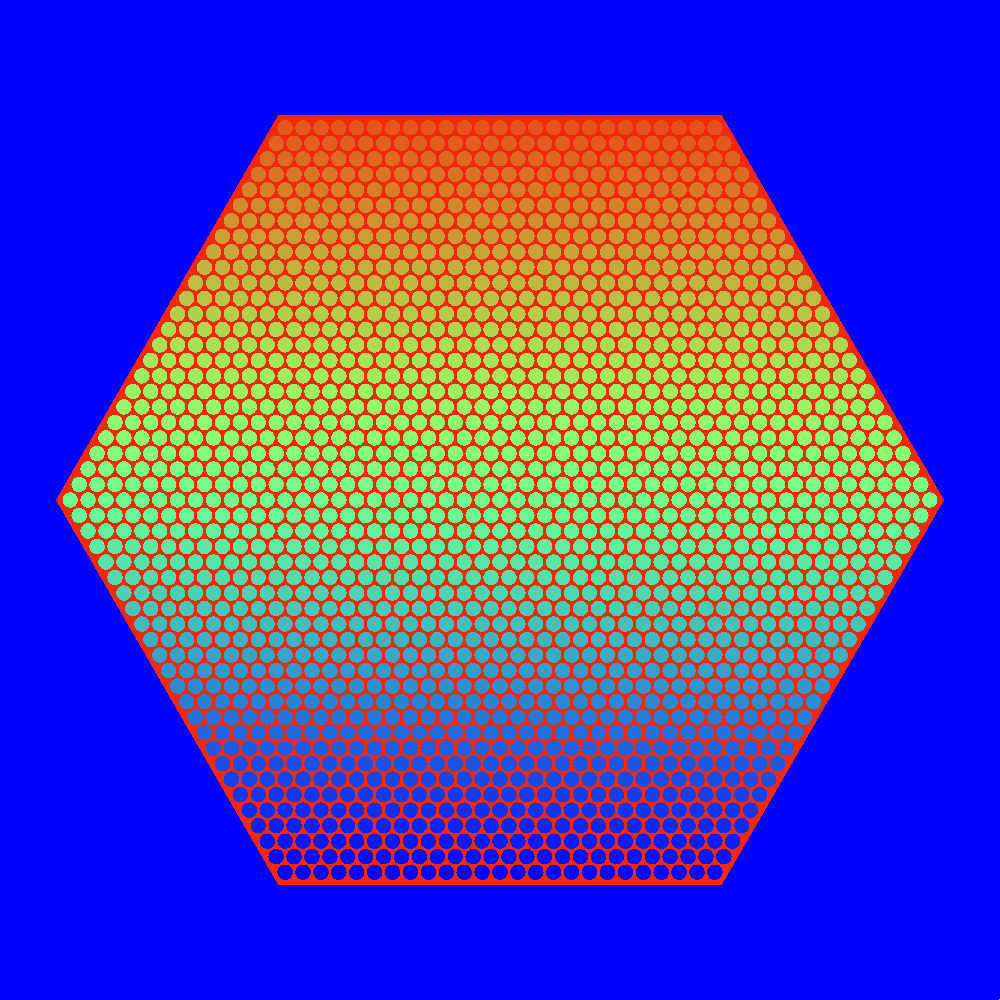
\includegraphics[width=.9\linewidth]{graphics/large_assembly.png}
  \caption{The large assembly}
  \label{fig:sub2}
\end{subfigure}
\caption{Raster images of $x$-$y$ cross sections of the geometry created by using the PIP cell/material query algorithm \label{raster_images}}
\label{fig:test}
\end{figure}

The cell numbers are mapped to colors in the image, and since there are no errors, it appears the routine is working and the algorithm can calculate the cell numbers.  A nice feature of OptiX is that variables can be attached to each geometry primitive.  In addition to the cell ID number, the materiel ID is also attached, so the material query can be done directly by OptiX rather than determining the cell number, then having to do an additional lookup or hash afterwards.

\subsubsection{Results}

Figure \ref{prelim_optix_k20} shows the ray trace rates for running these geometries on a NVIDIA Tesla K20 card.  There are cases for each geometry (assembly, large, and interleaved), whether the trace uses primitive or transform instancing (prim or xfrm), and whether it uses a split bounding volume hierarchy or regular bounding volume hierarchy (Sbvh or Bvh).  These traces all employed the cell number query PIP algorithm, so these rates are representative of the actual rates in a Monte Carlo Simulation where not only the first intersection must be found.  The source point distribution in all cases is uniformly random over all space and isotropically random in angle.  The trace rates are fairly constant after $10^6$ particles, but primitive instancing is always faster than transform instancing, and using BVH acceleration is always faster than SBVH.   The only time this isn't the case is for the interleaved assembly, where transform instancing performs slightly better than primitive instancing.  

\begin{figure}[h!] 
  \centering
    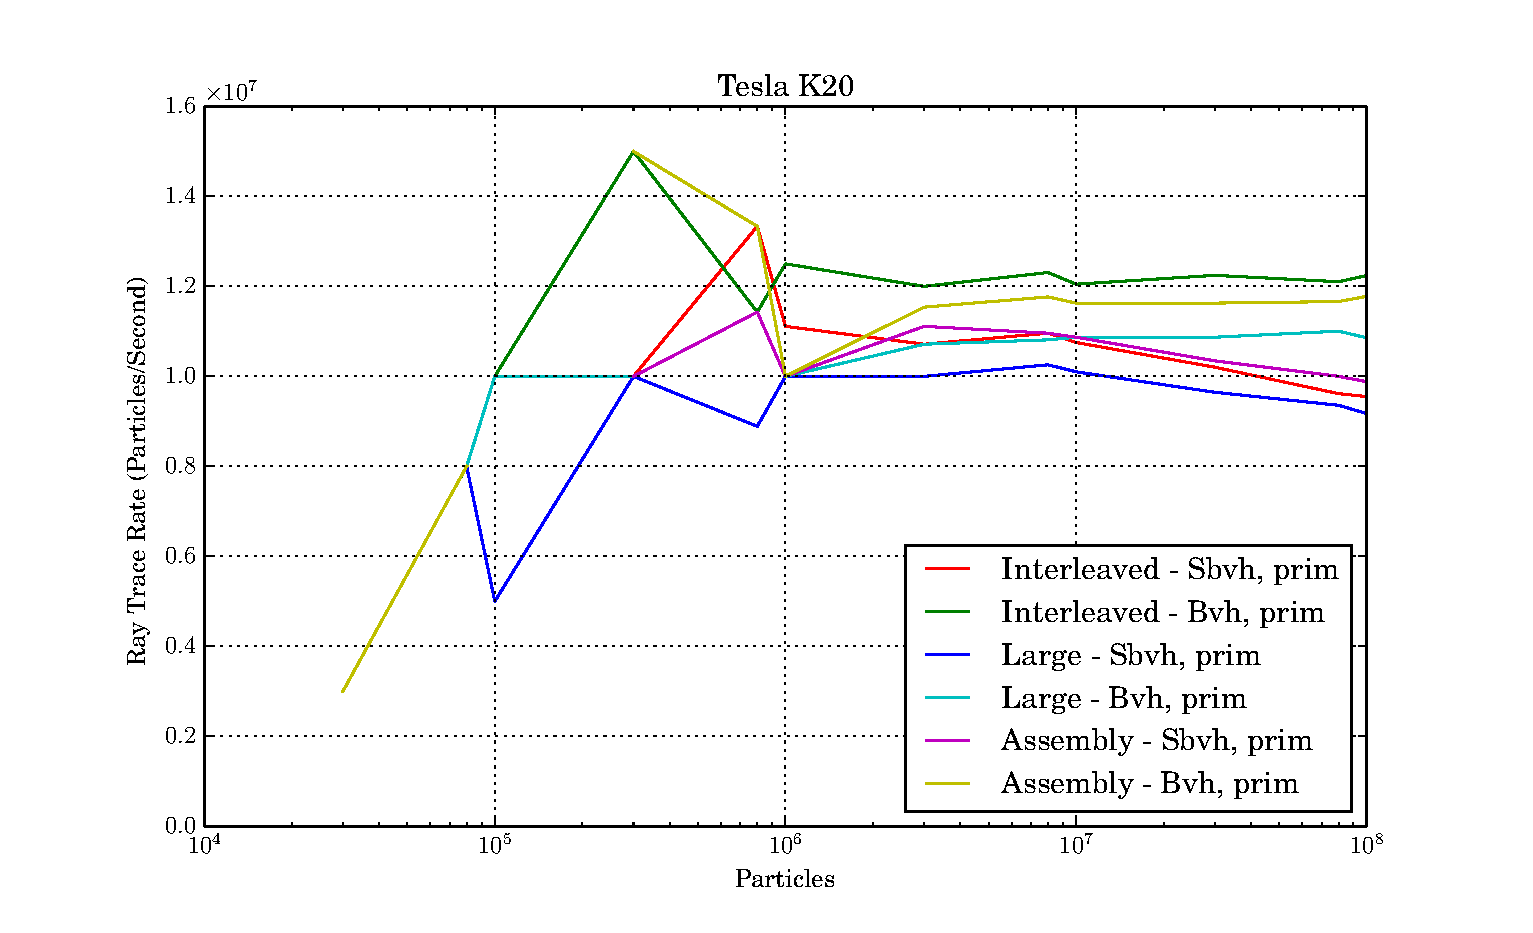
\includegraphics[width=0.8\textwidth]{graphics/prelim_optix_k20.eps}
     \caption{Trace rates of a NVIDIA Tesla K20 performing cell queries with the PIP algorithm. \label{prelim_optix_k20} }
\end{figure}

The interleaved assembly is also the geometry with the least amount of objects.  Another study was done to show the scaling of the two instancing types.  In these traces, a cell query was again done from a uniformly random and isotropic distribution of source points.  The number of source points was set to $8\times10^7$ for every trace in order to ensure being on the trace rate plateau shown in in Figure \ref{prelim_optix_k20}.  A BVH acceleration structure was also used, since this structure showed the best performance.  The geometry used was another hexagonal lattice of cylinders, identical to the assembly and large assemblies test geometries, only with more elements.  The volume, pitch to diameter ratio, and aspect ratios of the large cells were kept constant, but the cylinder radii were halved while doubling the number of elements on a edge.  Figure \ref{prelim_optix_scaling} shows the results of the scaling test, and it can be seen that XXX.  Traces were also done in a cell containing no objects, and rates were on the order of ten times faster,

\begin{figure}[h!] 
  \centering
    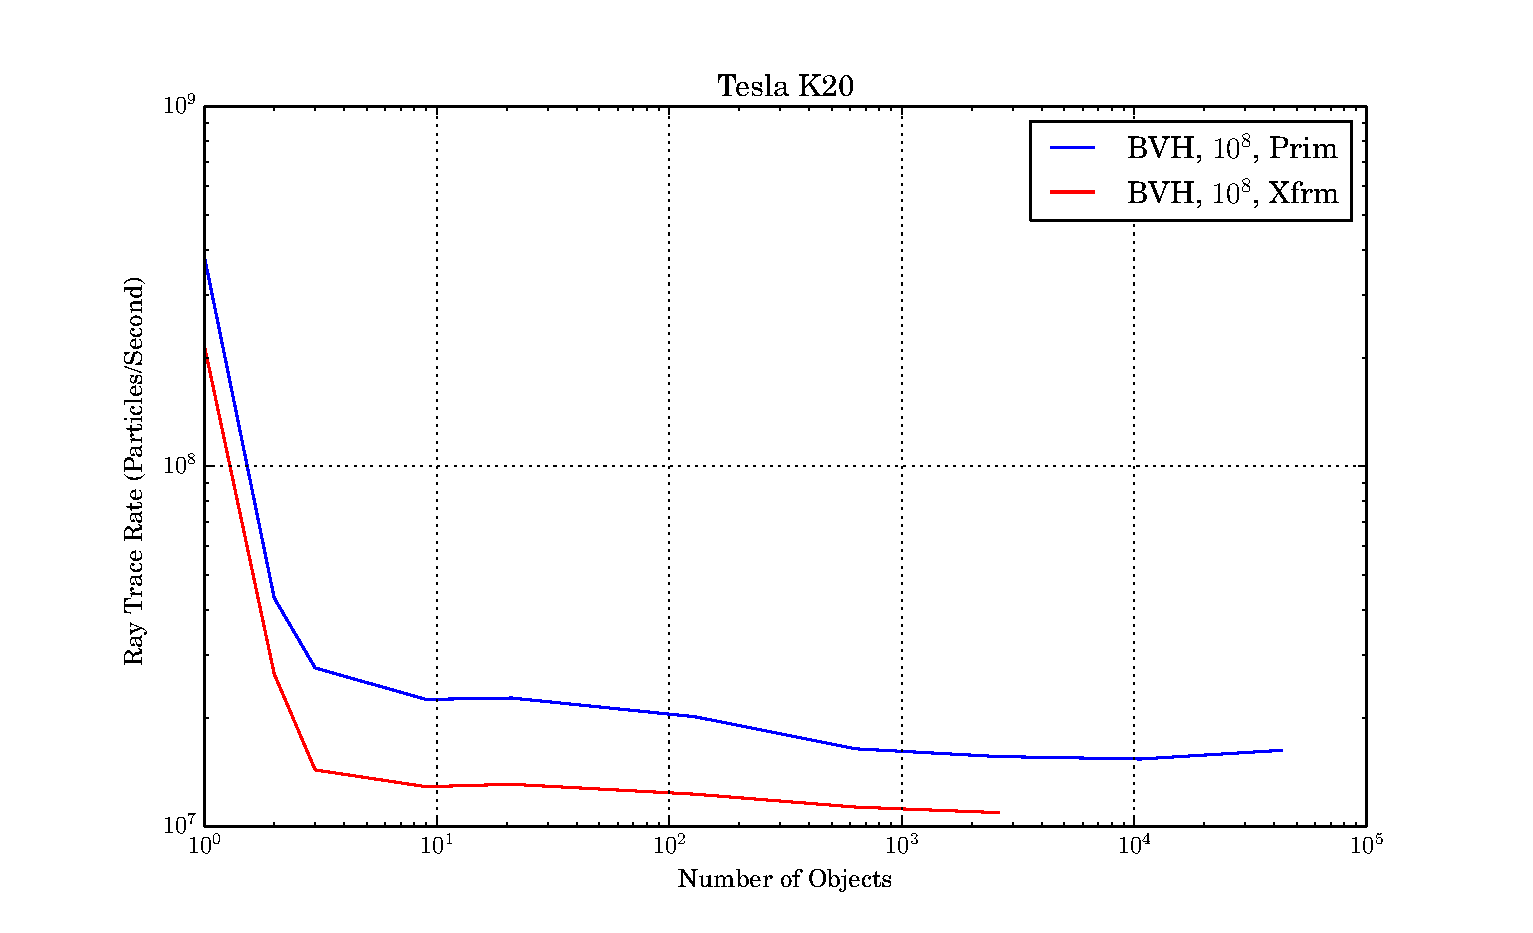
\includegraphics[width=0.8\textwidth]{graphics/prelim_optix_scaling.eps}
     \caption{Trace rate scaling on a NVIDIA Tesla K20 performing cell queries with the PIP algorithm. \label{prelim_optix_scaling} }
\end{figure}

Using transform instancing did not work for cell numbers above XXX cells.  Host memory consumption became too great and the process would be terminated.  This is why transform instancing trace stops at XXX cells in Figure \ref{prelim_optix_scaling}.  Structure construction prior to the trace also became very slow, presumably due to the independent acceleration objects attached to every instance and the overhead of computing all the affine transformations at acceleration structure build time.

Also, traces were done where the direction of every particle was in the negative $z$ direction, since this is the direction with the fewest number of surfaces between the source particles and the boundary cell.  Performance was increased marginally, but this can only be taken advantage in geometries where there is a direction of least heterogeneity (like lattices).

Figure \ref{prelim_optix_G650M} shows the same benchmark, but run on a NVIDIA GeForce GT 650M, the discrete graphics card in a MacBook Pro, Mid-2012 Retina model.  The same trends can be observed, except that overall trace rate is much slower, which is not surprising, and that the impact of transform instancing is very pronounced in runs with fewer particles.  This study was done to simply show the performance of a smaller, non-compute card compared to that of the Tesla card.

\begin{figure}[h!] 
  \centering
    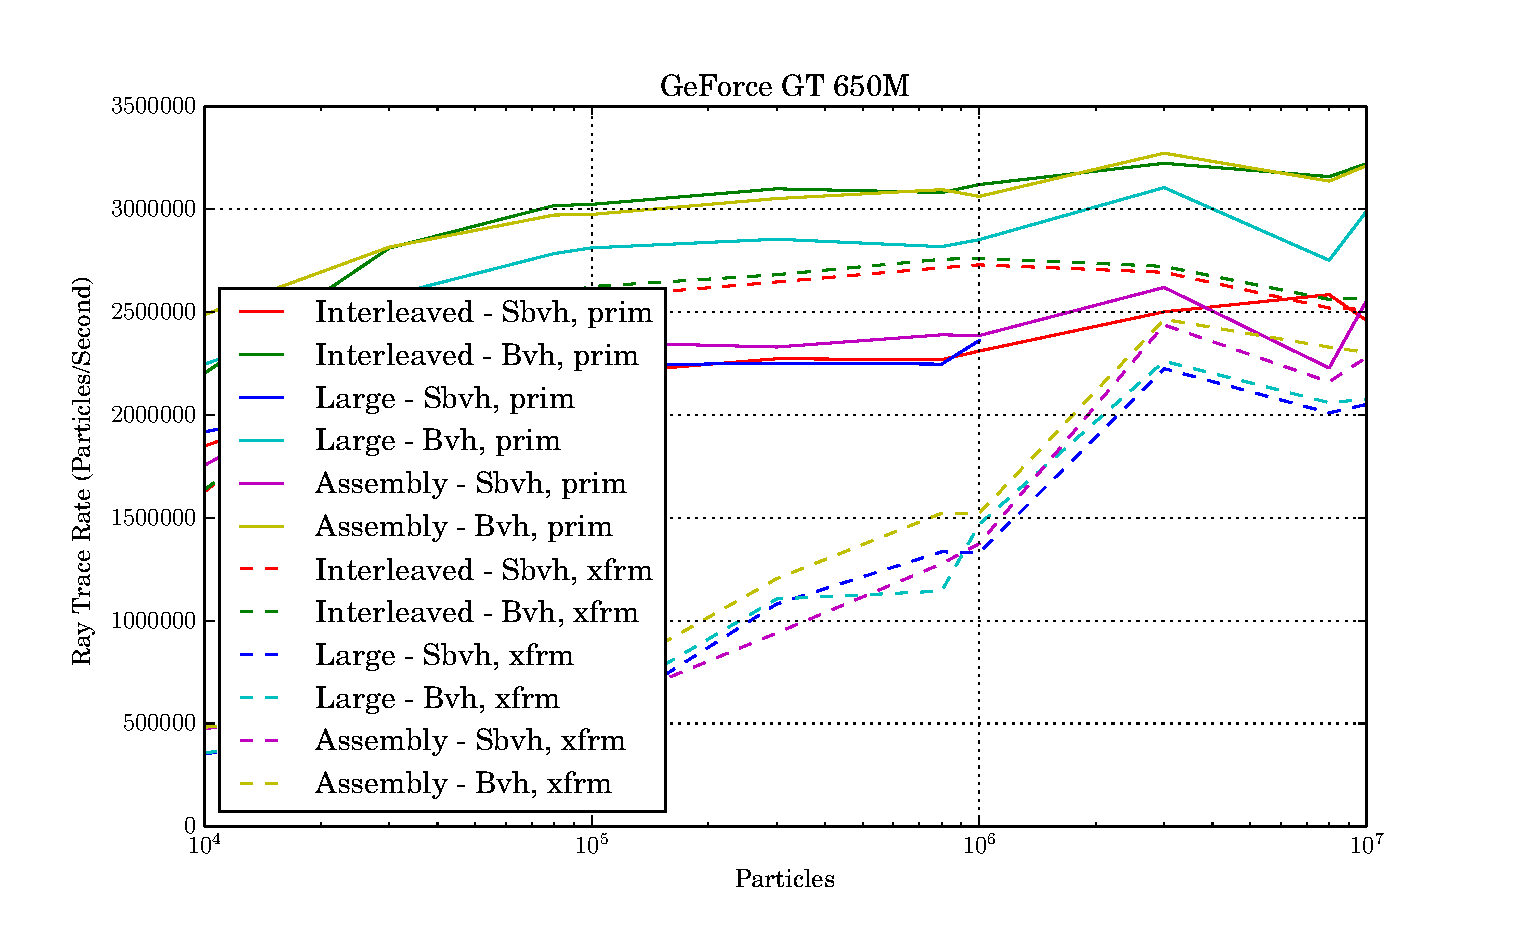
\includegraphics[width=0.8\textwidth]{graphics/prelim_optix_G650M.eps}
     \caption{Trace rates of a NVIDIA GeForce GT 650M performing cell queries with the PIP algorithm. \label{prelim_optix_G650M} }
\end{figure}

%%%%%%%%%%%%%%%%%%%%%%%%%%%%%%

\section{WARP in Detail}

The preliminary studies show that thread divergence can be effectively reduce with CUDPP without incurring huge costs, large datasets need to be run in order to hide memory latency, and a BVH acceleration structure in OptiX performs best for randomly-oriented distributions of rays.  Since most data will be access randomly no matter what, the layout will be regularized as much as possible and the particles will be sorted by reaction, sweeping out completed particles and grouping similarly-interacting particles together to maximize warp coherence and occupancy.  Since histories complete randomly, history data access will become sparse even if sweeping out is not done, and the radix sort will preserve monotonically increasing thread IDs within a reaction group, so it's impact on data access should be small, and the only cost be that of performing the operation.

As stated before, WARP will read ACE-formatted data, perform all reaction types as prescribed by them, use a Serpent-like unionized energy grid to regularize data access, use an event-based transport algorithm with parallelized operations for sorts and sums, use OptiX for general 3D geometry representation (without explicit nesting), use a SOA for neutron history data, and perform all operations on the GPU unless strictly forbidden.  From here on, it will be expanding the preliminary studies.  OptiX will be used for 3D geometry representation, physics routines that use real cross section data will be made in CUDA, the compaction routine in CUDPP will be substituted for a radix sort, tallies will be implemented, as will criticality and fixed source methods.  These expansion will yield WARP, a program for continuous energy Monte Carlo neutron transport on GPUs in general 3D geometries, which will be compared for accuracy and execution speed against Serpent and MCNP.

WARP will be written in C/C++ with some Python (which will be explained later in this section), and will rely on the OptiX framework for geometry representation and the CUDPP libraries for dataset-wide parallel operations. Single precision floating point number will be sued throughout in order to realize the full computational capacity of the GPU and to allow simulations to be carried out on more affordable and higher clocked GeForce cards.  Double precision is only needed XXX \cite{please}.

At this point, all the geometry routines are have been described in detail and the subsequent sections will discuss the cross section data access patterns and the energy related routines.

%%%%%%%%%%%%%%%%%%%%%%%%%%%%%%

\section{Data Layout}

As described in Chapter \ref{chap:background}, the nuclear data required in Monte Carlo simulations is very heterogeneous.

\subsection{Unionized Cross Sections}

It is particularly troublesome that each cross section has its own independent energy grid.  Using point-wise data for continuous energy simulations requires an interpolation be performed between points, and to do this, the code must somehow scan the energy grid array to find the points between which the neutron's energy falls.  If every isotope has its own grid, this search must be done for every isotope, and can become very expensive.  This is why the unionized energy grid structure, like that implemented in Serpent, is used by WARP.

Unionizing the cross sections simply means that the energy grids of the cross sections are all unionized into a single, larger vector which every isotope can use.  Doing this makes holes the the data, however, but these are filled by linear interpolation.  Since linear interpolation is always used to interpolate the cross sections, no information is lost and the cross sections are preserved.  The resulting dataset is larger than the sum of the individual cross sections, however, since it contains redundant data.  This is the tradeoff between regularizing the data in this way as opposed to accessing the energy grids separately.  Figure \ref{unionized_layout} shows the unionization process with two small, arbitrary energy grids and their corresponding cross section vectors.

\begin{figure}[h!] 
\centering
\includegraphics[width=0.5\textwidth]{graphics/unionized.eps}
\caption{Unionizing two cross section vectors. \label{unionized_layout} }
\end{figure}


unionized glory, why its good and bad \cite{jaakko}.

constant memory, not much improvement according to nelson

\subsection{Distribution Data as Linked Lists}

\begin{figure}[h!] 
\centering
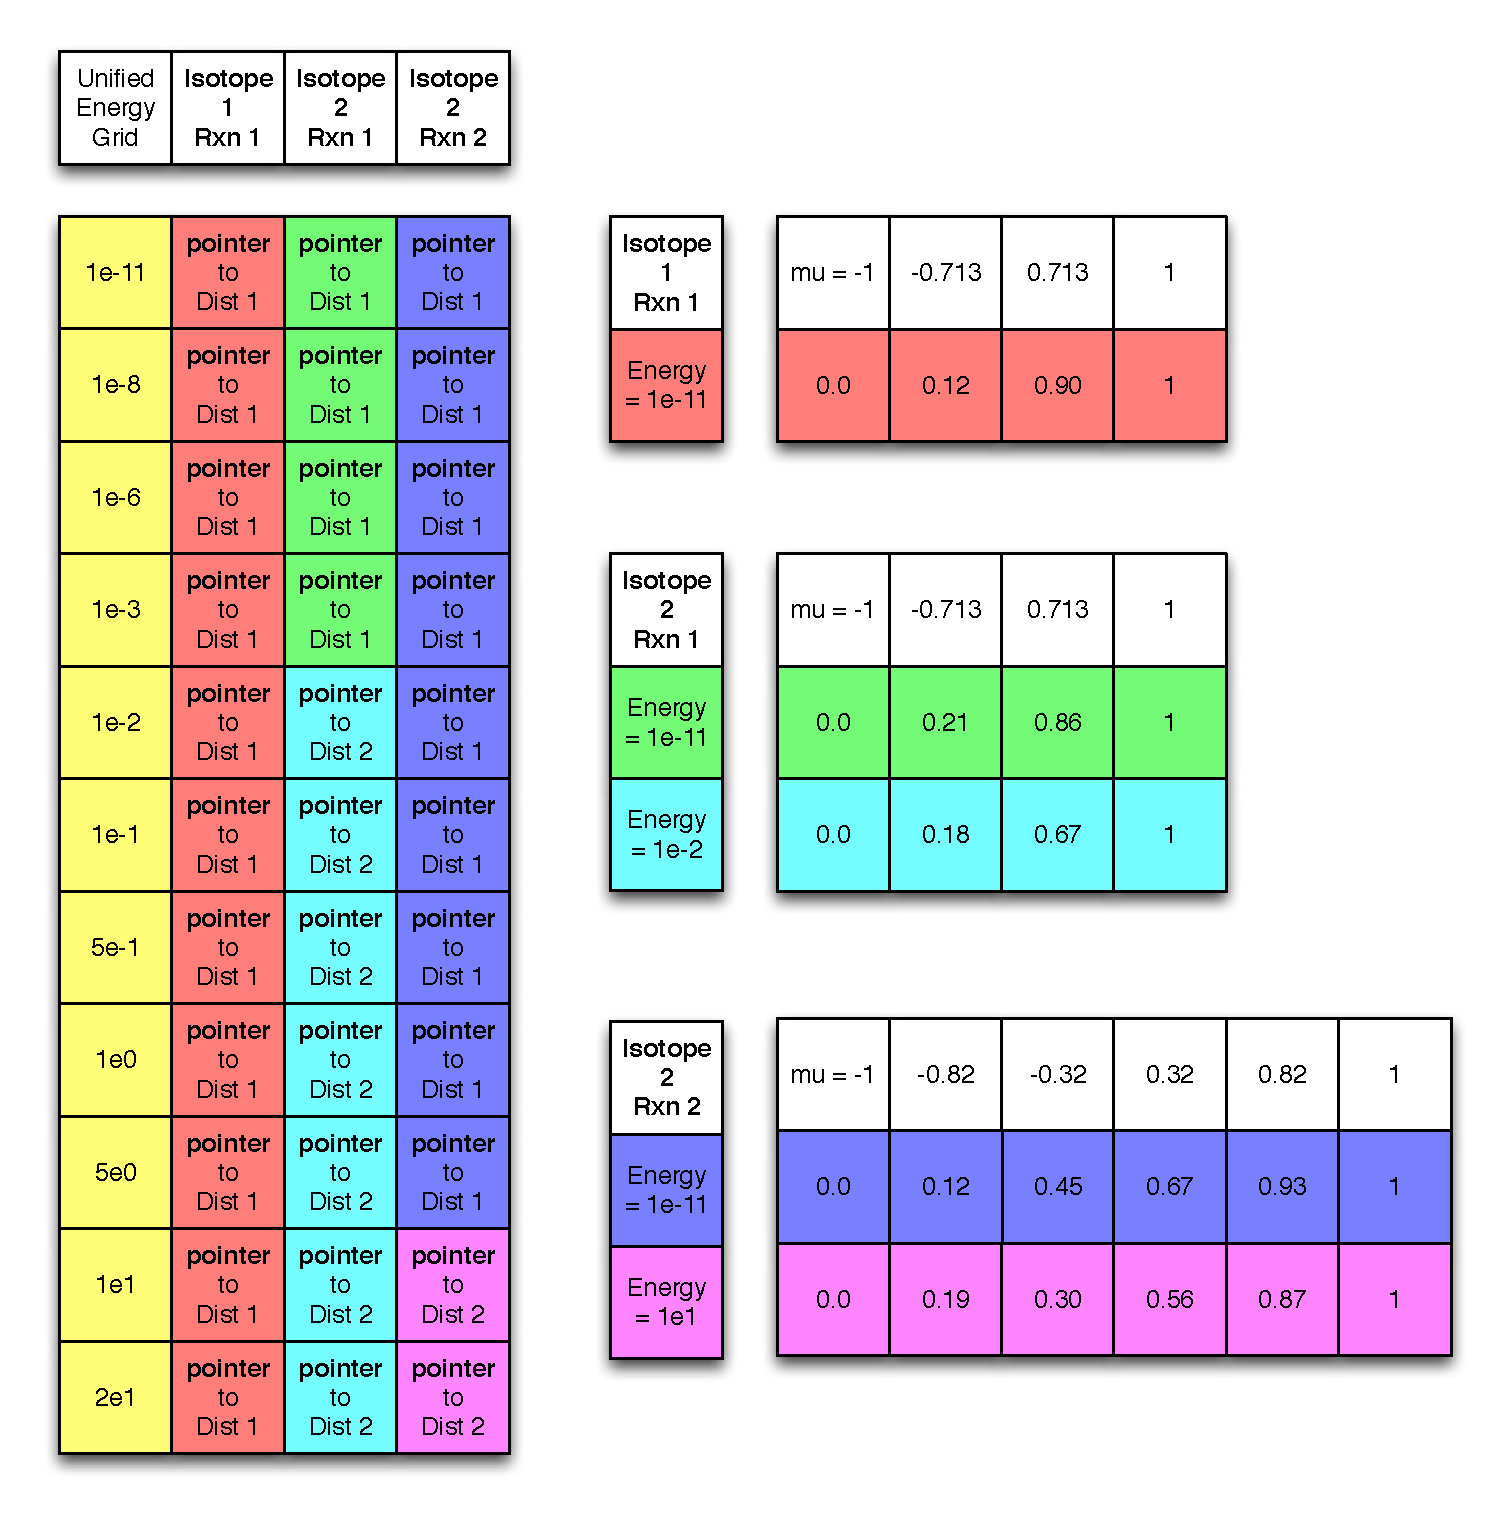
\includegraphics[width=0.7\textwidth]{graphics/unionized_pointers.eps}
\caption{Making a link to distribution data in the unionized dataset. \label{unionized_pointers} }
\end{figure}

how to resolve the data heterogeneity problem without having massive data replication

float4, have to implement, should be relatively easy

\subsection{Embedded Python}

PyNE

amazing Python C API

not using S(a,b) or unresolved resonance parameters at this point

%%%%%%%%%%%%%%%%%%%%%%%%%%%%%%

\section{Tasks}

\begin{figure}[h!] 
\centering
\includegraphics[width=0.9\textwidth]{graphics/warp_pipeline.eps}
\caption{WARP transport loop. \label{warp_pipeline} }
\end{figure}


breakdown of tasks into sub-tasks, actually going through how data is stored, accessed, etc

\subsection{Grid Search}

It is convenient that the values are monotonically increasing, but since the array is composed of floating point values with arbitrary spacing, an inverse function cannot made to calculate an index in $O(1)$ time.   A naive approach would be to scan the array from be beginning, performing comparisons along the way, and therefore calculating the cross section array index in $O(n)$ time, where $n$ is the number of elements in the array.

binary search here? more logN?  quad tree?  approximate function for initial guess?

\subsection{Geometry Representation}

stuff about geom and "where am I?"

\subsubsection{OptiX}

details about ray tracing, how a hit program works

\subsubsection{Acceleration Structures}

Importance of logN


\subsubsection{Scaling}

geometry instancing performance tests

optix scaling toy problem - need to have very large sets in order to hide overhead


\subsection{Pseudo-Random Numbers}

use of rejection sampling disqualifies precomputation of random number, plus it is very bandwith intensive to do so!

using lcrng keeps global access down and improves performance greatly

\subsection{Macroscopic}

material

\subsection{Microscopic}

nuclide

\subsection{Interactions}

\subsubsection{Scattering}

Rodriguez rotation

\subsubsection{Secondary-Producing}


\subsubsection{Disappearance}


\subsubsection{Concurrent Kernels}

\subsection{Parallel Operations}

CUDPP, reductions, sums, and sorts - sorting by reaction to keep warps full, memory implications

\subsubsection{Fixed source subcritical multiplication}

necessary to be subcritical.

pop can pop source particles in to keep population constant until NPS exceeded...

\subsubsection{Criticality}

cannot simply pop, unless generation number is associated, then data can be generated and post-processed?

does pop work in supercritical?

need to do generations since the source update is generation-dependent, can this be changed?





